\documentclass[conference]{IEEEtran}

\usepackage{amsmath}
\usepackage{graphicx}
\usepackage{subfigure}
\usepackage{color}
\usepackage{xspace}
\usepackage{url}
\usepackage[utf8]{inputenc}

\newcommand{\lorem}               {\textcolor{green}{Lorem ipsum dolor sit amet, consectetur adipisicing elit, sed do eiusmod tempor incididunt ut labore et dolore magna aliqua. Ut enim ad minim veniam, quis nostrud exercitation ullamco laboris nisi ut aliquip ex ea commodo consequat. Duis aute irure dolor in reprehenderit in voluptate velit esse cillum dolore eu fugiat nulla pariatur. Excepteur sint occaecat cupidatat non proident, sunt in culpa qui officia deserunt mollit anim id est laborum.}}
\newcommand{\smip}                {SmartMesh~IP\xspace}
\newcommand{\rpi}                 {Raspberry~Pi\xspace}

\graphicspath{{figs/}}

\begin{document}
\title{Talk to a Flower to Become a Part of the Internet}

\author{
    \IEEEauthorblockN{
        Ivana~Jovanovic,
        Márton~Sebestény,
        Mario~Zelić,
        Keoma~Brun-Laguna,
   }
}

\maketitle

\begin{abstract}
On the Summer School of Science 2016 in Pozega on S3++ camp we have been given a problem about an automated watering system for plants.
The goal of our project is to make a completely automated system which provides water to a plant according to its needs.
We solved the problem by making a circuit which involves a water pump and a moisture sensor that are connected to an Arduino Nano.
Arduino Nano controls the water pump according to the data it gets from the moisture sensor.
The produced data is sent to Raspberry Pi from where it is displayed on a web page.
\end{abstract}

\begin{IEEEkeywords}
Smart Agriculture, Precision Agriculture, IoT.
\end{IEEEkeywords}

\IEEEpeerreviewmaketitle

%==============================================================================
\section{Overview}
\label{sec:overview}

% problem

Everyday a huge amount of plants die because of lack of attention and love.
People go into holiday or simply forget due to their constant stress.

% current solutions

The final product can water the plants in apsense of humans and keep them hydrated.

% our system/product

The goal of the project is to establish an automated system that waters the plant according to its needs without any human intervention.
The whole product has three main sections:
i) the moisture measurement
ii) the automated water pumping
iii) and the server for self-hosting.

% measurements

The moisture sensor measures conductivity of the soil.
The more water there is, the higher the connductivity.
Although, a problem may occur if there is a high amount of metal ions, from the soil itself or accumulated over time from water.
It represents a possible problem because it can effect the conductivity of the soil and cause a higher measurement.
It sends the analog data to the small computer capable of prossesing the data and storing a small software in it.

% water automation

More precisely, we use Arduino Nano as "small, complete, and breadboard-friendly board"~\footnote{https://www.arduino.cc/en/Main/ArduinoBoardNano} for storing and executing our software.
The code is written in C/C++ like language.
The software in Arduino processes the data from the sensor, determines if the value is above or under the defined limit and enables the pump to water the plant if the value is low.
The limiting value for the pump is defined according to the type of the plant and the type of the soil becouse they effect the conductivity of the soil wich is measured.
Arduino and the pump together are powered by an external battery via USB port.

% self-hosting

At the same time Arduino sends the data from the moisture sensor to the Raspberry Pi via radio frequency.
Raspberry Pi is a small computer similar to the Arduino but more powerful.
It has an Ethernet port for connection to the internet.
We use it as web server which stores our data and displays it like a graph in a form of a web page.
Using the web server we can monitor the system from the distance and easily see the current state of the plant according to the graph.
The Raspberry Pi has it's own power source.

% conclusion of the intro

Our prototype is a turn-key solution currently applicable to personal needs.
The main advantages are the facts that it does not consume a lot of energy and that the whole product is self-contained.

\begin{figure}
    \centering
    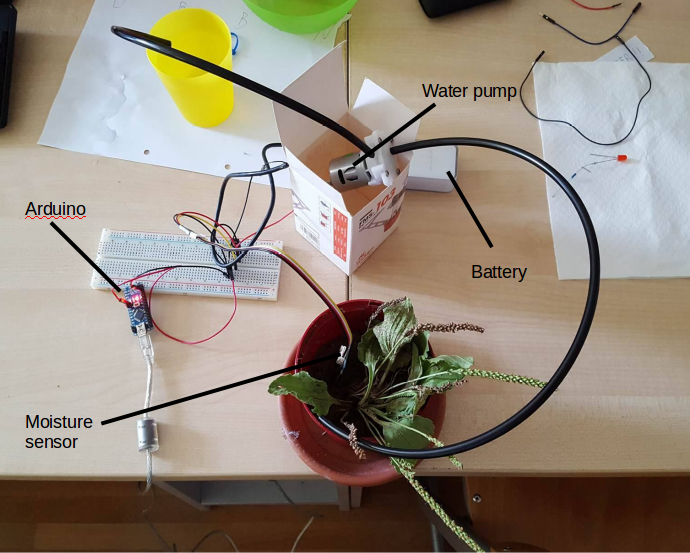
\includegraphics[width=\columnwidth]{prototype}
    \caption{A plant connected to the automated watering system.}
    \label{fig:prototype}
\end{figure}

%==============================================================================
\section{Automated Watering}
\label{sec:automated}

Our automated watering system consists of two major parts:
one which is responsible for collecting data about the soil and one which brings off the watering.
The device that joins the two parts is the Arduino Nano.

%------------------------------------------------------------------------------
\subsection{Measuring Moisture}

% hardware

To measure the soil moisture we use the following devices:
moisture sensor, Arduino Nano, a 5V battery and cables to connect them.
To make the system work we use an Arduino code (the Arduino language is based on C/C++) which controls the other parts of the circuit.

% conductivity

Our sensor measures the electrical conductivity of the soil and sends an analog signal to the Arduino Board.
The sensor we use provides analog values that can vary between 0 and 1024.
If we put the sensor in the air, we get a 0 as it's conductivity is very low in ordinary circumstances (i.e 10 to the power of -15).
If we make a shortcut with a cable between the two pins of the sensor, we get the maximum value as the cable has negligible resistance.
To calibrate the maximum humidity we put the sensor in water and at room temperature, this value is about 900.
If we want to calibrate the minimal humidity in our soil we need to dry it and measure the conductivity of the dry material.
Due to time limitation we consider the minimal value to be 0.
According to this data we can calculate the relative moisture percentage of soil and meet the plants water needs.

%------------------------------------------------------------------------------
\subsection{Watering System}

Our watering system contains a waterpump, a transistor (NPN), a diode, a battery and everything is connected to our Arduino Board.
We use the transistor as a switch and the diode as a safety mechanism.
Based on the data that our sensor provides, the Arduino Nano decides (thanks to our code) wether the plant needs water.
According to that it can close the circuit of the water pump for a certain amount of time (by using our transistor) and make the pump push water to the soil.
If it happens, we wait for a short time so the water can spread and then the whole process starts again.
If it does not happen, then the measurement continues.

\begin{figure}
    \centering
    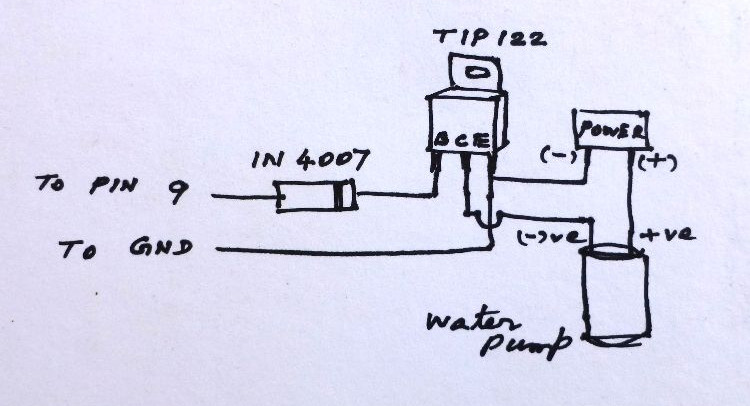
\includegraphics[width=\columnwidth]{circuit}
    \caption{The Watering electronical circuit.}
    \label{fig:circuit}
\end{figure}

%==============================================================================
\section{Data Collection and Hosting}
\label{sec:collection}

% intro

Now that the automated system for watering a plant is completed, we want to be able to store and analyze the data.
To do so, we establish a communication between the Arduino Nano and the Raspberry Pi.
Once that is done, we start modifying the software for the Raspberry Pi which writes the recieved data into a file.
Next step is designing the web page and displaying the data on a graph.

%------------------------------------------------------------------------------
\subsection{RF Communication}

Our automated system is controlled by an Arduino Nano which activates the pump according to the information it recieves from the moisture sensor.
To improve the performance of our system and find the optimal settings, we decide to save the data on a server and analyze it.
To communicate between the Raspberry Pi and the Arduino Nano, we are using a radio transmitter and a reciever.
Our radio transmitter and reciever use the 433 MHz frequency to send and recieve data.
We use an existing solution(footnote) to recieve the data that we then adapt to save both time and value into a comma-separated value (CSV) file.

% OOK

To effectivly transfer the data, we use on/off keying.
On/off keying is a type of digital modulation which represents data as a series of 1-value and 0-value that represent presence or absence of the carrier wave.
Another type of modulation is analog modulation which can be amplitude modulation (AM) and frequency modulation (FM).
Our Arduino Nano is equipped with a transmitter which either emits or does not emit waves which are recognized by a reciever connected to the Raspberry Pi as 1-value and 0-value.
When the server recieves the data, it translates the series of binary digits into useful information which represents the data sent from the Arduino Nano.
After that, the time when the data was recieved is remembered and if it satisfies all the conditions, the data is saved.


% interferences

By using radio transmission of the information, we are exposed to different types of interferences.
When waves are travelling from the transmitter to the reciever, there is a probability that some data can be lost.
To decrese the probability of data loss, we send the same data three times in a very small timeframe (<1s).
After the data is sent, Raspberry Pi usually recieves multiple packets of data that were sent.
Since the same data is recieved more than once, we only need to store one packet of data and the rest we can discard.
We pick which data to store by modifying the existing solution.
We set conditions which need to be satisfied.
The conditions are: the value of the data must not be 0, and the time the packet was recieved must not be the same as the time the last packet was recieved.

%------------------------------------------------------------------------------
\subsection{Hosting}

% Web server

After the database is set up, we display the collected data on a web page.
The web page needs to contain a graph which represents the relative amount of moisture of soil over time and some additional information about our project.
We decide to use Python to create a web server, HTML for the content and CSS for the style.

%==============================================================================
\section{Reproducible Research}
\label{sec:reproducible}

% description

One of the main goals of this project is to show the importance of reproducible research.
This is a kind of research which can be repeated after the initial research.
Currently, this is a big problem in the science community since a lot of research is being done, but not all of them can be repeated.
This is due to unspecified procedures which were used during the research and/or insufficient information about the used equipment and the result of the research.

% version control

One of the most popular ways of making research reproducible is using a version control system.
Version control system is a system which is used for remembering all versions of the research.
It remembers the difference between two versions of the same part of the research so the changes are visible and easily readable.
Saving all versions of the research contains data of successes and failures.
This way the same mistakes cannot be made since there are already notes on how they happened and how they could be stopped.
Version control systems encourage originality in a way that they have the option of "branching".
Branching is an event which happens after the research is split into more parts and they concentrate on different aspects of the problem.
This is a useful concept since every branch can access the data which was collected before branching, but cannot see the information other branches have collected.
Not all research can use a version control system because of the amount of data, complexity of the procedures or the type of research.

% git

On our project, we used Git as a version control system on which we saved all files connected to the project\footnote{\url{https://github.com/keomabrun/S3\_2016}}.
Every time we change something, we send the changes we made in our repository on Github ("push") so the current version is saved.
When the changes are monitored, we can see what was the problem and how we solved it.


%==============================================================================
\section{Conclusion}
\label{sec:conclusion}

% project description

In the Summer School of Science (S3++) our team got an opportunity to take part in a practicle, Computer Science project.
Our main purpose was to set up an automatic watering system with which we succeeded.
Meanwhile we learnt a lot about programming, electronics, Computer Science in general and also about many other fields of science (including Physics and Chemistry).
We assembled an all-in-one automatic watering system and documented in a step-by-step approach so that it can be reproduced by anyone for a few kunas.

% further improvements

Further improvements include:
i) adding additional temperature and humidity sensors,
ii) analysing the interaction between the different metrics,
iii) collecting data about different plants
iv) adding a user friendly interface.

\begin{figure}
    \centering
    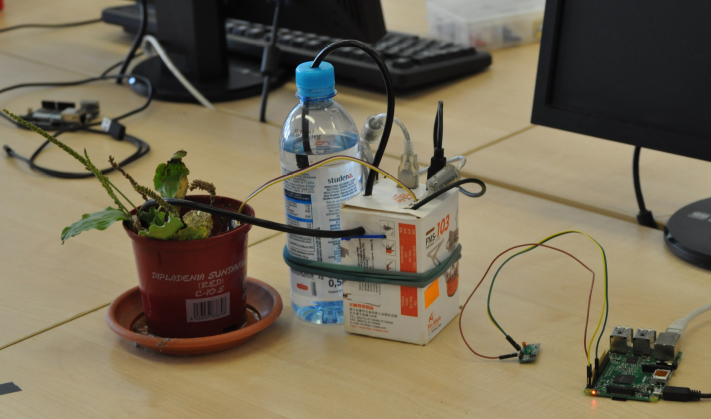
\includegraphics[width=\columnwidth]{final_box}
    \caption{The Watering electronical circuit.}
    \label{fig:final_box}
\end{figure}
%==============================================================================
\section*{Acknowledgments}

% Summer School Organisation

We would like to greatefully thank the organizers of the Summer School for their help and constant support.

% Maja for the water testing

We want to thank Maja for her presence and advices during the water testing process.
We also want to thank Davor and Boris for their experience sharing in electronics.

%==============================================================================

\bibliographystyle{IEEEtran}
\begin{thebibliography}{10}
    \bibitem{}
\end{thebibliography}

\end{document}
